\section{Stability, and timing in detail}\label{app:gain}
\sectionstate{partial}{\texttt{rerun/paper1\_timeseries} (Runs 1 and 2 against time), \texttt{rerun/paper1\_timing} (timing; the
old section 8 and appendix F), \texttt{rerun/paper1\_res} (resolution against drift field); corrections from
\texttt{papers/paper1\_v2/NUMBERS\_RUNDOWN.md} item 1 and \texttt{figs/out/gain\_scan.json}. v2 2026-11-10: the stability figure
existed and was unused.}
\intent{This appendix answers: is the chamber stable over ten hours, and what does the time resolution depend on?}

\subsection{Runs 1 and 2 against time}
\Cref{fig:timeseries} follows chamber~A through its two long runs. Charge, efficiency, position, angle and time
resolution are flat over the ten hours and agree between the runs: the angular resolution is 0.975 and
0.991\textdegree{} in X and 0.896 and 0.900\textdegree{} in Y, the uncorrelated time 22.4 and 22.2\,ns. The one
quantity that moves is the drift velocity. Measured on one estimator, the angle-scale velocity anchored to the timing
velocity of Run~1, it is 35.8\,\textmu m/ns in Run~1 and 36.4\,\textmu m/ns in Run~2, rising from 36.2 to 36.6 during
the night: $+1.8\,\%$, as the water falls from 0.99 to 0.94\,\% (\cref{sec:drying}).
\askDylan{The old text had ``35.8 against 37.2\,\textmu m/ns''. Those were two different estimators (Run~1's timing velocity;
Run~2's velocity with the angle-scale factor folded in), and 37.2 is by coincidence also the top of the field scan.}
\begin{figure}[tbp]
  \centering
  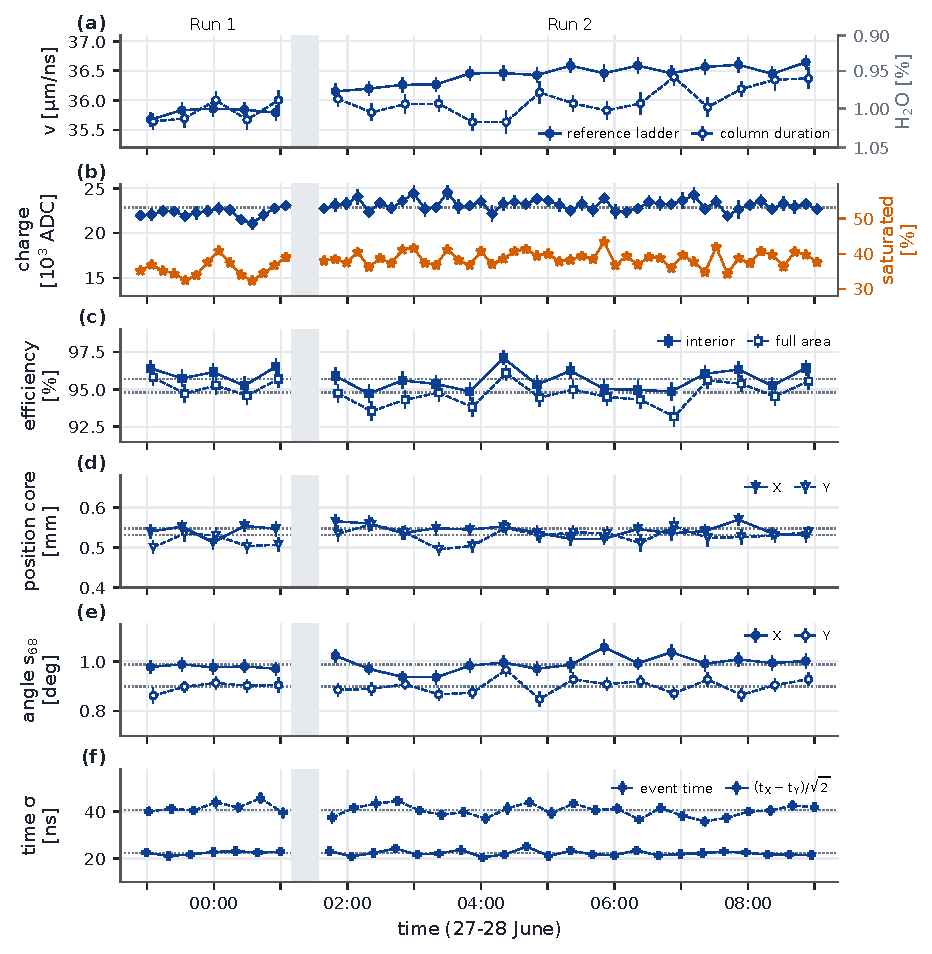
\includegraphics[width=\linewidth]{det_a_timeseries}
  \caption{Chamber~A through Runs 1 and 2 (night of 27--28 June), in bins of time. (a) Drift velocity from the
  reference tracks and from the duration of the drift column and, right axis, the water it corresponds to. (b) Median
  track charge and the fraction of saturated tracks. (c) Efficiency in the interior and over the full area. (d) Core of
  the position residual. (e) Angular resolution. (f) Time resolution. X filled, Y open. Dotted lines: the mean of each
  run.}
  \label{fig:timeseries}
\end{figure}

\subsection{Angular resolution against drift field}
At 490\,V, in the drift-field scan of chamber~A, the angular resolution stays between 0.92 and 0.97\textdegree{} in X
and 0.87 and 1.00\textdegree{} in Y from 167 to 367\,V/cm, with about 650 tracks per point; at 100\,V/cm, where the
drift column no longer fits in the readout window, it is 2.0\textdegree.

\subsection{Time resolution: what it depends on}\label{app:timingdetails}
\Cref{fig:timing} shows the time resolution of chamber~A against the size of the early signal, the sum over strips of
the amplitude at the rising edge from which the time is read. Every scan point lies on one curve, and Runs 1 and 2,
binned in that amplitude at one voltage, lie on the same curve (within 0.89--1.01 of it). The time resolution is
therefore set by the signal over the noise. Time walk is not what limits it: a correction for the median time against
amplitude moves the event time of Runs 1 and 2 from 40.7 to 40.5\,ns and leaves the uncorrelated part at 22.3\,ns.

Against the drift field at 490\,V (\cref{fig:timing_driftscan}) the event time falls from 114 to 79, 52, 41, 42 and
38\,ns as the field rises from 106 to 177, 248, 319, 355 and 390\,V/cm, and the uncorrelated part from 46 to 22\,ns.
Converted to drift distance with the timing velocity of each point, the event time is 1.3--1.5\,mm at every field from
177 to 390\,V/cm, and the part common to the two views 1.2--1.4\,mm. Against the field, then, the time resolution is a
depth, roughly constant, divided by a velocity that grows with the field. The scan does not say where in the chamber
that depth comes from.

\Cref{fig:timing_all} gives the same quantities for all chambers.
\begin{figure}[tbp]
  \centering
  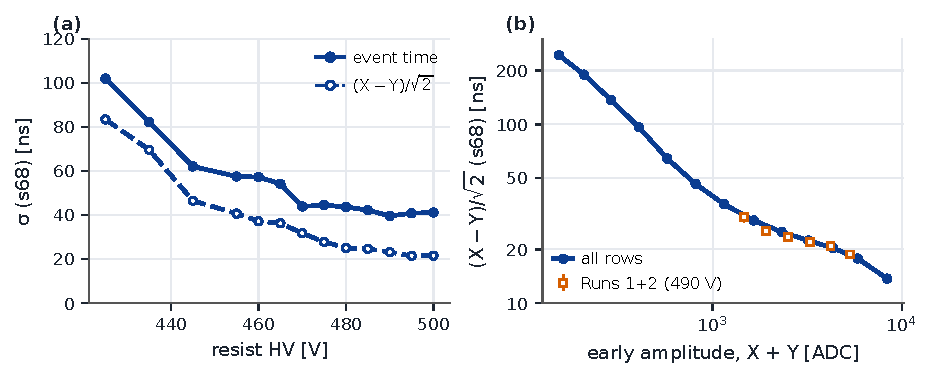
\includegraphics[width=\linewidth]{timing}
  \caption{Time resolution of chamber~A for reference-matched cosmic tracks ($s_{68}$): (a) against $HV_\mathrm{resist}$
  in the scan of 27 June, the event time and the uncorrelated part $(t_X-t_Y)/\sqrt2$ (the same data as
  \crefp{fig:gainscan}{d}); (b) the uncorrelated part against the size of the early signal, for all scan points and for
  Runs 1 and 2.}
  \label{fig:timing}
\end{figure}
\begin{figure}[tbp]
  \centering
  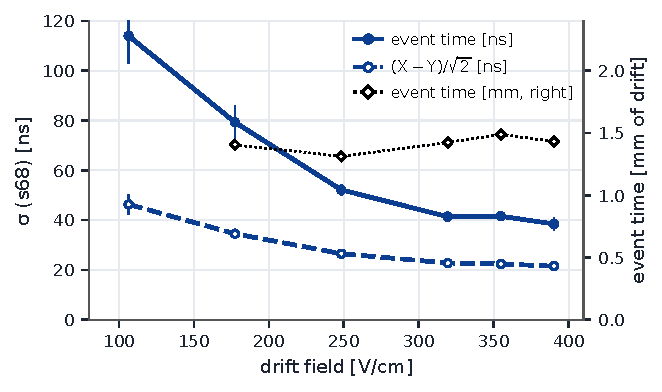
\includegraphics[width=\linewidth]{timing_driftscan}
  \caption{Time resolution of chamber~A against the drift field at 490\,V (reference-matched tracks, $s_{68}$). (a) Event
  time (solid) and $(t_X-t_Y)/\sqrt2$ (dashed) in ns. (b) The event time in mm of drift (not available at
  106\,V/cm, where the column overruns the readout window). Error bars: statistical.}
  \label{fig:timing_driftscan}
\end{figure}
\begin{figure}[tbp]
  \centering
  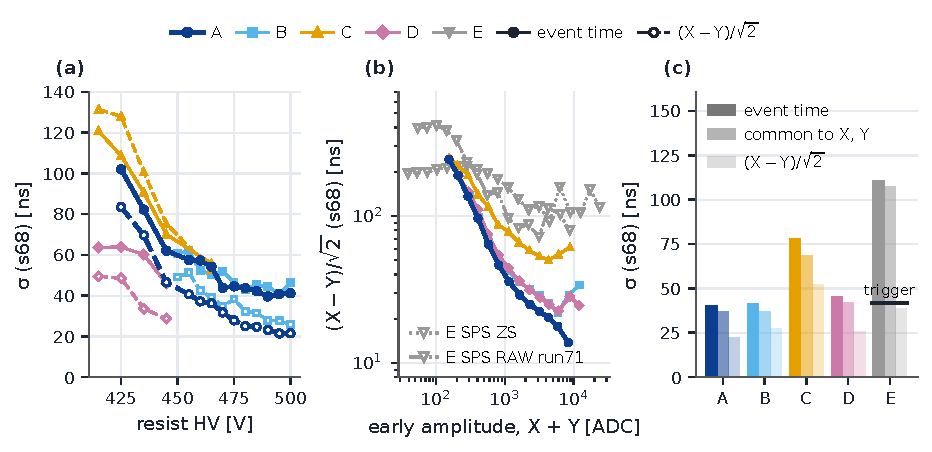
\includegraphics[width=\linewidth]{timing_all}
  \caption{Time resolution on the bench for all chambers: (a) event time (solid) and uncorrelated part (dashed)
  against $HV_\mathrm{resist}$ in the scans; (b) the uncorrelated part against the size of the early signal, with
  chamber~E in the beam (open grey); (c) on the long runs, the event time, the part common to X and Y, and the
  uncorrelated part.}
  \label{fig:timing_all}
\end{figure}
\askDylan{\Crefp{fig:timing_all}{a} is drawn from all clean triggers, not reference-matched tracks, so below 465\,V it lies above
\crefp{fig:gainscan}{d} (the 109 against 83\,ns disagreement of the audit). It should be remade on matched tracks or lose panel (a).
Its caption also had ``the trigger term is 42\,ns (chamber~E)'', which nothing in the text explained; dropped.}
